\scrollmode                    % To exit upon error
\documentclass[letterpaper,twoside,12pt]{article}
\usepackage{polyglossia}
\setmainlanguage{russian}
%\setmainfont{Times New Roman} % Change to another font if Times New Roman fails
\newfontfamily\cyrillicfont{Times New Roman} % Specify the Cyrillic font

\usepackage[margin=0.8in]{geometry}
\usepackage{amsmath}
\usepackage{unicode-math} % For Unicode math support
\usepackage{graphicx}

%\title{\text{Расчёт выделения тепла в бухте-удлинителе}}
\title{Расчёт выделения тепла в бухте-удлинителе}

\author{Бенкевич Л. В.}

\begin{document}

\maketitle 

\emph{Задача.} Нагреватель воды мощностью $P = 2200 \text{Вт}$ подсоединён к сети напряжением $U = 220 \text{В}$ через удлинитель, длинный двужильный кабель длиной $l = 50 \text{м}$ и сечением каждой из двух жил $a = 0.75 \text{мм}^2$. Кабель-удлинитель смотан в бухту (размеры и число витков не имеют значения, пусть будет диаметр ~ 20-30 см). \\

Найти тепловую мощность, выделяемую в бухте кабеля.


\begin{figure}[h]
    \centering
    \begin{minipage}{0.45\textwidth}
        \centering
        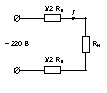
\includegraphics[width=\linewidth]{circuit_Rb_Rn_Rb.pdf}
        \caption{Сопротивления одной жилы кабеля, $\frac{1}{2} R_\text{Б}$, нагрузки (нагревателя воды), $R_\text{Н}$, и другой жилы кабеля, $\frac{1}{2} R_\text{Б}$,  в бухте.}
        \label{rb_rn_rb}
    \end{minipage}
    \hfill
    \begin{minipage}{0.45\textwidth}
        \centering
        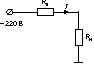
\includegraphics[width=\linewidth]{circuit_Rb_Rn.pdf}
        \caption{Сопротивления обеих жил кабеля в бухте, $R_\text{Б}$, и нагрузки (нагревателя воды), $R_\text{Н}$.}
        \label{rb_rn}
    \end{minipage}
\end{figure}


%\begin{figure}[ht!]
%%  \begin{center}
%  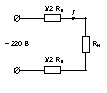
\includegraphics[width=20pc]{circuit_Rb_Rn_Rb.pdf}
%  \caption{\small \text{Сопротивления одной жилы кабеля, нагрузки (нагревателя воды) и другой жилы кабеля в бухте.}}
%  \label{rb_rn_rb}
%%  \end{center}
%\end{figure}

\emph{Решение.} Заметим, что ток последовательно протекает через три сопротивления (Рис.~\ref{rb_rn_rb}): жилу кабеля, $\frac{1}{2} R_\text{Б}$, сопротивление нагревателя воды, $R_\text{Н}$, и возвращается через другую жилу кабеля, $\frac{1}{2} R_\text{Б}$. Сначала найдём все сопротивления, затем ток через них, а потом – мощность $P_\text{Б}$, выделяемую этим током в бухте.

Поскольку последовательные сопротивления складываются, мы можем эту схему упростить, заменив эквивалентной, состоящей из полного сопротивления бухты, $R_\text{Б}$, и нагревателя, $R_\text{Н}$ (Рис.~\ref{rb_rn}):

%\begin{figure}[ht!]
%  \begin{center}
%  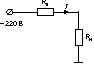
\includegraphics[width=20pc]{circuit_Rb_Rn.pdf}
%  \caption{\small \text{Сопротивления обеих жил кабеля в бухте и нагрузки (нагревателя воды).}}
%  \label{rb_rn}
%  \end{center}
%\end{figure}



Полное сопротивление кабеля в бухте, то есть последовательное сопротивление обеих жил $R_\text{Б}$ определяется удельным сопротивлением меди, 
$\rho = 0.0172 \frac{\text{Ом мм}^2}{\text{м}}$, его сечением $a$ и длиной $l$:     % \text{Ом мм^2}

\begin{equation}
  \label{rbuh}
  R_\text{Б} = \rho\frac{l}{a}.
\end{equation}


\begin{equation}
  \label{ohm_law}
  I = \frac{U_{220~\text{В}}}{R_\text{Б} + R_\text{Н}}
\end{equation}

Здесь $U_{220~\text{В}}$ обозначает напряжение, $R_\text{Б}$ — сопротивление бухты сетевого кабеля, а $R_\text{Н}$ — сопротивление нагрузки


\end{document}

